\documentclass[11pt,a4paper]{article}
\usepackage[margin=2.4cm]{geometry}
\usepackage[T1]{fontenc}
\usepackage{lmodern,microtype}
\usepackage{amsmath,amssymb,booktabs,enumitem,xcolor,graphicx,tabularx}
\usepackage[colorlinks=true,linkcolor=blue!50!black,urlcolor=blue!50!black]{hyperref}
\setlist{itemsep=2pt,topsep=3pt}
\newcommand{\E}{\mathbb{E}}
\newcommand{\Var}{\operatorname{Var}}
\newcommand{\Cov}{\operatorname{Cov}}
\newcommand{\Law}{\operatorname{Law}}
\newcommand{\sg}{\operatorname{sg}}
\newcommand{\tr}{\operatorname{tr}}
\newcommand{\N}{\mathcal{N}}
\newcommand{\status}[1]{\textsf{\small\color{black!60}[#1]}}
\newcommand{\head}[1]{\par\smallskip\noindent\textbf{#1}\ }
\title{Improving Few-Step Conditional It\^o Maps:\\ Diagnosis and Research Ideas Worth Continuing}
\author{Internal research note}
\date{23 November 2026}
\sloppy
\begin{document}
\maketitle

\noindent\textbf{Scope.} This note collects ideas for improving the conditional It\^o-map forecaster of the manuscript \emph{Few-Step Probabilistic Forecasting with Conditional It\^o Maps} and its implementation in \texttt{src/scisi}. It targets three goals: quality at 1--4 sampling steps, stability of long autoregressive rollouts, and physics (or other) consistency. Only ideas that survived a novelty search, a derivation check and, where cheap, a numerical check are kept; the rest are listed in Section~\ref{sec:discarded} with reasons.

\medskip\noindent\textbf{How it was produced.} Five agents worked in parallel: one each on few-step sampling, rollouts and physics consistency, a literature scout, and one running toy experiments. Their full reports and scripts are in \texttt{agent\_reports/} (Appendix~\ref{sec:provenance}).

\medskip\noindent\textbf{Status labels.} \status{derived}: derivation only. \status{toy}: confirmed on a scalar or 1D toy. \status{data}: measured on the stochastic Navier--Stokes archive. \status{unverified}: plausible but unchecked. Nothing here was run on a trained Navier--Stokes map. Novelty statements rest on targeted searches, many at abstract level.

\section{Summary}

The central finding is a diagnosis. The map's only random input is a per-pixel white martingale, and its covariance is mismatched to the forecast uncertainty by about four decades across wavenumbers. The network must therefore amplify noise at the forced scales and cancel it at small scales, through a zero-initialised feature branch that is never supervised by data. This accounts for most of the known failure modes (Section~\ref{sec:diagnosis}).

The unifying thesis for the fixes is: \emph{put the uncertainty and the physics into the martingale}. Its covariance should be the forecast uncertainty, its null space the invariants, its conditioning the observations, and its trace the energy budgets.

\begin{table}[h]
\small
\begin{tabularx}{\linewidth}{@{}lXll@{}}
\toprule
 & Idea & Goal & Novelty / evidence\\
\midrule
A & Covariance-matched martingale with matched schedule $\beta_t=t\sqrt{3-2t}$ & few-step & new criterion; \status{toy}, \status{data}\\
B & Weak closure: energy-score self-distillation conditional on the coarse path & few-step & new combination; \status{derived}\\
C & Picard self-distillation (random-node integral target) & few-step & not found; \status{derived}\\
D & Interpolant refresh: law-preserving one-call corrector, used in training and inference & rollout & new guarantees; \status{derived}\\
E & Chapman--Kolmogorov closure with direct-lead teachers & rollout & moderate; \status{derived}\\
F & Stationary window matching on persistent chains & rollout & modest; \status{derived}\\
G & It\^o-budget consistency (weak physics residual for an SPDE) & physics & not found; \status{data}\\
H & Invariant-closed maps and driver & physics & low, exact; \status{derived}\\
I & Martingale Kalman conditioning in path space & physics / DA & new; \status{derived}\\
J & Forcing-revealed latents (needs regenerated data) & physics & not found; \status{unverified}\\
\bottomrule
\end{tabularx}
\caption{Kept ideas. A is the recommended first step and several others depend on it.}
\end{table}

\noindent Three directions I expected to be contributions are not. Legendre path features and terminal energy-score fine-tuning are prior art but helped in the toy study and should be adopted. The exponential-integrator (bridge) form of the map did not help and is not recommended (Sections~\ref{sec:hygiene} and~\ref{sec:toy}).

\section{Diagnosis}\label{sec:diagnosis}

\begin{center}
\includegraphics[width=\linewidth]{figures/fig_diagnosis.pdf}\\[2pt]
{\small\itshape Left: per-wavenumber power of the one-step increment relative to the white driver (data). Right: spread of a map that ignores the path, for a Gaussian surrogate with $a=0.1$ (toy).}
\end{center}

\head{Setting.} The forecasting SDE is $dX_t=b_t(X_t;h)\,dt+\gamma_t\,dW_t$, $X_0=c(h)$, $\gamma_t=a(1-t)$, with interpolant $I_t=(1-t)c+\beta_ty+\gamma_t\sqrt t\,z$. The map is $\Phi_{s,t}(x)=x+(t-s)G_\theta(s,t,x,h;\Psi_{s,t})+M_t-M_s$ with $M=\int\gamma\,dW$ and $\Psi$ a finite path description.

\head{A one-step map is a conditional-mean generator.} Since $X_0=c$ is deterministic, $\Phi_{0,1}=c+G_{0,1}(\Psi)+M_1$ is a noise-to-data generator whose squared-error optimum is $\E[X_1\mid\Psi]$. The explicit martingale contributes white spread $a/\sqrt3$ per pixel. Everything else must come from the learned $\Psi$-dependence of $G$, which enters through a zero-initialised $1\times1$ projection, vanishes on the diagonal and is only bootstrapped by self-distillation. Any shortfall regresses the map towards a path-ignorant, Euler-like map.

\head{The driver is spectrally mismatched \status{data}.} In normalised coordinates, the per-mode power of the one-interval increment $y-c$ (an upper bound on the conditional variance) relative to $\Var(M_1)=a^2/3$ is

\begin{center}\small
\begin{tabular}{lcccccccc}
\toprule
Shell $|k|$ & 1 & 4 & 7 & 11 & 16 & 32 & 48 & 64\\
\midrule
increment / white & 0.31 & 20 & 190 & 59 & 9.8 & 0.59 & 0.066 & 0.012\\
\bottomrule
\end{tabular}
\end{center}

\noindent The forced shells are under-noised by about $10^2$ and the small scales over-noised by about $10^2$. The table was computed for one value of $a$; changing $a$ shifts all entries by a constant factor and leaves the four-decade range.

\head{Which regime the code is in.} The current training grid uses $a=1$ (the default in \texttt{config/models/ito\_map.yaml}; \texttt{config/stochastic\_navier\_stokes.yaml} does not override it). Other configs, and possibly the archived initial-stage runs, use $a=0.1$. With $a=1$ the per-pixel martingale variance is $0.33$ against a forecast-error variance of roughly $0.03$ (inferred from old CRPS values; rough), so the network must cancel about $90\%$ of the noise it is handed. With $a=0.1$ it must instead create most of the variance. Both regimes share the scale mismatch above.

\head{Path-ignorant limit \status{toy}.} For a Gaussian surrogate $y\mid h\sim\N(m,\sigma^2)$ with $a=0.1$, $\sigma=0.17$, $\beta=t^2$, an Euler-drift map with exact noise has endpoint std$/\sigma$ of $0.34,\,0.58,\,0.65,\,0.78,\,0.88,\,0.97$ at $N=1,2,4,8,16,64$ steps. The multi-step solver reference is itself underdispersed at finite $N$, and a 32-step rollout teacher caps the student below one.

\head{What this explains.}
\begin{itemize}
\item \emph{Underdispersion}: under-learned path dependence loses variance with a definite sign.
\item \emph{High-wavenumber spectral error}: a small relative cancellation error leaves a flat-spectrum residue, which the identity skip then passes on at every physical step.
\item \emph{PSD alone was insufficient, teacher rollout helped}: rollout supplies the path-dependent target directly; PSD must bootstrap it through many levels.
\item \emph{$K=16$ did not beat $K=4$}: in the Gaussian surrogate, four increments of $M$ already capture over $99\%$ of the linear response, so information is not the bottleneck there (the toy study in Section~\ref{sec:toy} qualifies this for multimodal targets).
\item \emph{The Gaussian-base flow map wins at one step}: there the noise is the state and the regression target is a deterministic function of the inputs.
\end{itemize}

\head{Further observations.}
\begin{itemize}
\item \emph{KL features cannot cancel the noise at intermediate budgets} \status{toy}. With $K=4$ global Karhunen--Lo\`eve coefficients and $a=1$, the part of the last step's martingale increment not explained by the features is $0.03\%$ at $N=1$ but $14.7\%$, $29.3\%$ and $79.7\%$ at $N=2,4,8$. This is a candidate cause of the non-monotone quality in step count for KL-feature maps.
\item \emph{KL train/sample mismatch} \status{derived}. Training draws $x=I_s$ independently of the global coefficients, but at sampling $X_s$ depends on $W_{[0,s]}$, which is correlated with them.
\item \emph{Non-nested splits} \status{toy}. With the split $u\in[0.25,0.75]$ the parent's four local increments are not functions of the children's eight ($R^2$ between $0.75$ and $0.91$), so even conditional kernels have no exact semigroup. Midpoint splits or Legendre moments are nested.
\item \emph{Loss weighting} \status{derived}. For $\beta=t$, average-drift MSE equals denoiser-space MSE times $1/(1-s)^2$; late-start intervals are weighted far more than $(0,1)$.
\item \emph{The flow decorrelates in about five snapshots} \status{data}. Field autocorrelation is $0.62$, $0.33$, $0.07$, $0.017$ at lags $1$, $2$, $5$, $10$. Any statement at lead $\geq8$ is about the chain's stationary law. ``Spread/skill $0.63$ at lead 10'' means either too little stationary variance or members that diverge too slowly, which need different fixes.
\item \emph{The energy and enstrophy budgets close on the archive to about $0.5\%$} \status{data}, and are consistent with $\nu=10^{-3}$, drag $\alpha=0.1$, forcing amplitude $\varepsilon=1$, spacing $\Delta=0.5$. This is evidence for the parameters listed as unknown, not a recovered manifest. A second agent, with a different palinstrophy estimate on the test split, found the enstrophy balance closing to $3.4\%$.
\end{itemize}

\head{Diagnostics to run first (no training).}
\begin{enumerate}
\item Per-wavenumber spread ratio of It\^o-1 against SI-128. Prediction: below one at forced scales, with a flat excess tail at high $k$.
\item Zero the path features at sampling in an existing checkpoint and measure the change in spread per shell.
\item Regress high-pass(sample) on high-pass($M_1$): a non-zero coefficient is leaked white noise.
\item Per lead: pooled member variance over climatology; member--member against member--truth pattern correlation (equal if calibrated); and a common-noise split, rerunning one step with a single shared Brownian path across members to separate injected from propagated spread.
\item The budget residual of idea G on existing rollouts, including beyond lead 95.
\end{enumerate}

\section{Few-step sampling}

\subsection*{A. Covariance-matched martingale (Gaussian-exact It\^o maps)}

\begin{center}
\includegraphics[width=\linewidth]{figures/fig_a.pdf}\\[2pt]
{\small\itshape Left: the white driver against the forecast uncertainty per wavenumber (data, relative units) and the proposed matched driver. Right: share of the endpoint variance the network must still supply (scalar toy).}
\end{center}

\head{Idea.} Choose the driver covariance and $\beta$ so that the martingale already \emph{is} the forecast uncertainty. The drift then becomes nearly state independent and the average drift nearly path independent, so the map has almost nothing to learn about the path. Two agents arrived at this independently, and I checked the algebra.

\head{Proposition \status{derived, toy}.} Let $I_t=(1-t)c+\beta_ty+\gamma_tC^{1/2}W_t$, $M=C^{1/2}\!\int\gamma\,dW$, $q(t)=\int_0^t\gamma_r^2dr$, and suppose $y\mid h\sim\N(m,\Sigma)$. If
\begin{equation}
C=\Sigma/q(1),\qquad \beta_t^2=\frac{q(t)-t\gamma_t^2}{q(1)},
\label{eq:matched}
\end{equation}
then $b_t(x;h)=-c+\dot\beta_tm$ for every $x$, $X_t=(1-t)c+\beta_tm+M_t$, and $G_{s,t}$ does not depend on the path. Every step count is exact with zero path features. The proof is one line: the drift target $R_t$ and $I_t$ are jointly Gaussian with $\Cov(R_t,I_t)=(\beta\dot\beta\,q(1)+t\gamma\dot\gamma)C=0$ by \eqref{eq:matched}. Equivalently, $\Var(I_t\mid h)=q(t)C=\Var(M_t)$: the interpolant's marginal variance runs on the martingale's variance clock.

For $\gamma_t=a(1-t)$ this gives, independently of $a$,
\[
\beta_t=t\sqrt{3-2t},\qquad \dot\beta_t=\frac{3(1-t)}{\sqrt{3-2t}},\qquad a_k=\sqrt3\,\sigma_k\ \text{per Fourier mode.}
\]

\head{Design criterion.} In general, choose $(C,\beta)$ to minimise $\int\E\|\nabla_xb_t(I_t)\|^2dt$. An It\^o map is one-step exact when its drift is spatially constant along the path; this is the stochastic counterpart of straight trajectories for ODE flow maps. \status{unverified beyond the Gaussian case}

\head{In practice.} Take $C$ Fourier-diagonal, equal to the mean conditional covariance $\bar\Sigma_k=\E_h\Var(\hat y_k\mid h)$, estimated from the residual of an MSE regressor or from anomalies of existing SI ensembles. Keep the full $(k_x,k_y)$ spectrum (the forcing is anisotropic), floor it, and set $C_0=0$. The variance clock, bridges, path features and both self-distillation losses are unchanged, because $C^{1/2}$ acts on the spatial index only. A history-dependent scale $C(h)=\lambda(h)^2C_0$ is allowed; $C$ must not be learned through the diagonal loss.

\head{Toy evidence \status{toy}.} Fraction of $\Var(X_1)$ not explained by $M_1$ alone (exact drift, scalar Gaussian-mixture targets):

\begin{center}\small
\begin{tabular}{lccc}
\toprule
Driver variance / target variance & $\beta=t^2$ & $\beta=t$ & matched $\beta$\\
\midrule
1 (Gaussian target) & 5.0\% & 1.2\% & 0.1\%\\
1 (skewed / bimodal) & 5.2 / 5.7\% & 1.3 / 1.4\% & 1.2 / 0.9\%\\
2 & 7.7\% & 3.5\% & 1.2\%\\
4 & 10.6\% & 6.9\% & 4.0\%\\
100 (today's high-$k$ regime) & 20--22\% & -- & 19--21\%\\
0.25 & 2.4\% & 4.6\% & 12.9\%\\
0.01 (today's forced-shell regime) & 13--17\% & -- & 64--69\%\\
\bottomrule
\end{tabular}
\end{center}

\noindent Covariance matching is the large lever (about $20\%\to1\%$). The matched $\beta$ helps for variance ratios in $[1,4]$ and hurts when the driver is under-noised. Rule: over-noise slightly, $C\approx1$--$2\times\bar\Sigma$, or keep $\beta=t$.

\head{Novelty.} Coloured noise is known in diffusion and flow models (functional flow matching, arXiv:2305.17209; EqualSNR, which colours by the \emph{unconditional} spectrum). Pan et al.\ (arXiv:2606.11156) and Strong Stochastic Flow Maps (arXiv:2606.01086) use white noise. Neither the schedule identity \eqref{eq:matched} nor path independence of the average drift as a selection criterion was found.

\head{Risks.} The conditional covariance is history dependent and not stationary in space. The conditional law may be far from Gaussian, since $\Delta=0.5$ exceeds a turnover time. It changes the process, so the SI baselines must be retrained on the same interpolant.

\head{Falsifier.} Train only the SI drift on the matched interpolant. If its Euler sampler at $N=1,2,4$ is still strongly underdispersed relative to its own $N=128$, or the nested Monte Carlo omitted-variance fraction at $K=4$ does not fall well below the $9.7\%$ in the lab notes, the idea fails. No map training is needed.

\head{Code.} A \texttt{MatchedStochasticInterpolation} in \texttt{models/interpolations.py}; a spectral multiplier at the single white draw in \texttt{\_WeightedPathBase.\_randn} and in the trainer's noise draws; the same multiplier in the baseline stepper.

\subsection*{B. Weak closure: energy-score self-distillation conditional on the coarse path}

\begin{center}
\includegraphics[width=\linewidth]{figures/fig_b.pdf}\\[2pt]
{\small\itshape Illustration with synthetic numbers. Given the resolved path features, the target is still random. A squared-error student returns its mean and loses that spread; an energy-score student with a latent reproduces it.}
\end{center}

\head{Idea.} Be pathwise on the $K$ resolved features and in-law on everything else. Give the network one extra white field $\eta$ and replace the off-diagonal MSE by a conditional energy score against the same composed EMA target $T$:
\[
\mathcal L=\E\Big[\tfrac12\textstyle\sum_{i=1,2}\|S(\eta_i)-T\|-\tfrac12\|S(\eta_1)-S(\eta_2)\|\Big],\qquad S(\eta)=G_\theta(s,t,x,h;\Psi_{s,t},\eta).
\]
The rule is strictly proper, so at the optimum $\Law(S\mid x,\Psi_{s,t})=\Law(T\mid x,\Psi_{s,t})$. Under-learned path dependence becomes mis-coupling instead of lost variance.

\head{Why it is principled \status{derived}.} With nested features, the true conditional kernels satisfy $Q_{s,t}(\cdot\mid x,\Psi_{s,t})=\E[Q_{u,t}\circ Q_{s,u}\mid\Psi_{s,t}]$, so they are an exact fixed point at every finite $K$. MSE-PSD has no such fixed point (the OU counterexample in the lab notes). Uniqueness given the diagonal is unverified. A data anchor fits the same loss: $\Law(\Phi_{0,t}(c;W,\eta))=\Law(I_t\mid h)$ for all $t$, scored against fresh interpolant samples; $t=1$ is ordinary CRPS on truth.

\head{Novelty.} Scoring-rule training of generators is well covered (distributional diffusion, arXiv:2502.02483; IMM, 2503.07565; Swift, 2509.25631; Tyche, 2605.06916; STMD, 2605.07661). New here: the score is conditional on a shared coarse Brownian path, with exact bridge refinement supplying the teacher's conditional randomness, inside two-time self-distillation. Terminal CRPS alone is \emph{not} novel and is the control.

\head{Risks.} The energy score is weakly discriminative in $128^2$ dimensions; use per-pixel fair CRPS plus a spectral or patch term. $\eta$ must vanish on the diagonal.

\head{Falsifier.} Fine-tune one checkpoint at equal budget with MSE-PSD, with this loss, and with terminal CRPS only. Drop it if rank histograms do not improve over the first, or if it adds nothing over the third at 2--4 steps.

\subsection*{C. Picard self-distillation}

\begin{center}
\includegraphics[width=\linewidth]{figures/fig_c.pdf}\\[2pt]
{\small\itshape Schematic. The progressive loss builds the parent target from two learned child maps. The Picard loss evaluates the data-trained drift at a random intermediate time.}
\end{center}

\head{Idea.} Teacher rollout worked because it evaluates the data-anchored diagonal along the path. The integral form of the Lagrangian identity does the same without simulation: $(t-s)G_{s,t}(x;W)=\int_s^tb_u(\Phi_{s,u}(x;W))\,du$, estimated with one random node $u\sim U(s,t)$,
\[
\mathcal L=\E\Big\|G_\theta(s,t,x;\Psi_{s,t})-\sg\Big[b_{\bar\theta}\big(u,\Phi_{\bar\theta,s,u}(x;W)\big)-\Big(\dot\beta_u-\tfrac{\beta_t-\beta_s}{t-s}\Big)y\Big]\Big\|^2 .
\]
The bracketed $y$ term has zero mean over $u$ and acts as a control variate. The cost equals PSD, no JVP is needed, and it works with local features.

\head{Mechanism \status{derived}.} Every target queries the diagonal. The target operator is of Volterra type, so idealised Picard iteration contracts factorially; the PSD operator passes child errors on with unit gain and never reaches the diagonal (gap floor $0.01$). The contraction is unverified for SGD.

\head{Novelty.} MeanFlow (arXiv:2505.13447) states the integral but differentiates it; the Lagrangian losses of Boffi et al.\ and Pan et al.\ are differential. No random-node integral target was found, from one search round.

\head{Falsifier.} Equal-budget comparison against PSD from the same diagonal checkpoint.

\subsection*{Adopt without claiming novelty}\label{sec:hygiene}

\begin{itemize}
\item \emph{Legendre path features, at their physical scale.} Shifted-Legendre moments of the increment process on $[s,t]$ are local, and a parent's moments are exact linear functions of the children's for any split \status{toy: residual $3.6\times10^{-15}$}. They are prior art: SSFM (arXiv:2606.01086) and iSSFM (arXiv:2610.29605) report Legendre beating KL. In the toy study (Section~\ref{sec:toy}) they were the clearest win: one-step error fell by a factor of 2--3 in every setting. Do not normalise features to unit variance; that hurt many-step accuracy.
\item \emph{Terminal energy-score anchor.} Scoring the one- and two-step outputs against data helped moderately in the toy (one-step $W_1$ down 25--40\%) at about $2.3\times$ training cost. Used without self-distillation it gives the best one-step law but a map unrelated to the SDE, which degrades with more steps.
\item \emph{Bridge (integrating-factor) form: not recommended.} For $\gamma=a(1-t)$ the drift is $b_t(x)=\kappa_t\hat y_t(x)-x/(1-t)$ with $\hat y_t=\E[y\mid I_t=x]$, hence
\[
\Phi_{s,t}(x)=\tfrac{1-t}{1-s}\,x+\Big[\beta_t-\beta_s\tfrac{1-t}{1-s}\Big]\bar Y_{s,t}+a(1-t)(W_t-W_s),
\]
with $\bar Y$ a weighted average of $\hat y$ along the path \status{toy: pathwise identity confirmed}. The explicit noise vanishes at $t=1$. I expected this to help; in the toy it was worse than the current form at every step count in four of five settings, and a repaired variant only matched the current form. The argument that the network ``must cancel $M_1$'' is also weaker than it looks in the toy, where $G_{0,1}$ is positively correlated with $M_1$ and has smaller variance than $X_1$. The toy has no spatial spectrum, so the high-wavenumber argument is untested, but idea A addresses that directly.
\item \emph{Midpoint (nested) splits, on-policy start states, gap floor to zero.} Known practice; midpoint splits are required by idea B.
\end{itemize}


\section{Toy study}\label{sec:toy}

A 1D two-mode Gaussian mixture, $c=0$, $a=1$, $\beta=t$, small MLPs, 20k updates, three seeds, 50k samples. The exact drift is closed-form, so a 2048-step reference exists; its own $W_1$ to the target is $0.014$, which is the floor. Features are $K=4$ unless stated.

\begin{center}\small
\begin{tabular}{lccccc}
\toprule
$W_1$ to target at $N$ steps & 1 & 2 & 4 & 8 & 16\\
\midrule
Current method (velocity form, local increments, PSD) & 0.126 & 0.030 & 0.022 & 0.015 & 0.014\\
\quad + energy-score anchor & 0.083 & 0.023 & 0.024 & 0.018 & 0.015\\
\quad with Legendre features & 0.039 & 0.026 & 0.031 & 0.028 & 0.022\\
\quad with Legendre features + anchor & 0.030 & 0.019 & 0.025 & 0.018 & 0.015\\
Bridge form as proposed & 0.179 & 0.079 & 0.068 & 0.073 & 0.084\\
Bridge form, repaired (skip) parametrisation & 0.177 & 0.046 & 0.022 & 0.015 & 0.016\\
Anchor only, no self-distillation & 0.024 & 0.033 & 0.046 & 0.076 & 0.100\\
Euler--Maruyama with exact drift & 1.042 & 0.343 & 0.143 & 0.075 & 0.042\\
\bottomrule
\end{tabular}
\end{center}

\noindent Seed standard deviations are $0.001$--$0.01$; differences below about $0.01$ are within noise.

\begin{itemize}
\item Legendre features halve the one-step pathwise error against the same-path reference ($0.44\to0.22$) and cut mode flips from $5.3\%$ to $1.7\%$. The gain is the same in both map forms, so it is a feature effect. The same factor of 2--3 at one step appeared with three modes, $a=0.5$, $\beta=t^2$ and a 2D mixture.
\item This qualifies the statement in Section~\ref{sec:diagnosis} that path information is not the bottleneck: that was derived for a Gaussian surrogate, and for a multimodal target the choice of features mattered.
\item The one-step defect of every self-distilled variant is a bridge of mass between the modes ($9.6\%$ of mass more than three standard deviations from any mode for the current method, $3.2\%$ with Legendre features, $0.3\%$ in truth).
\item The one-step standard-deviation ratio is $0.95$ for the current method, so the toy reproduces underdispersion only mildly.
\end{itemize}

\begin{center}
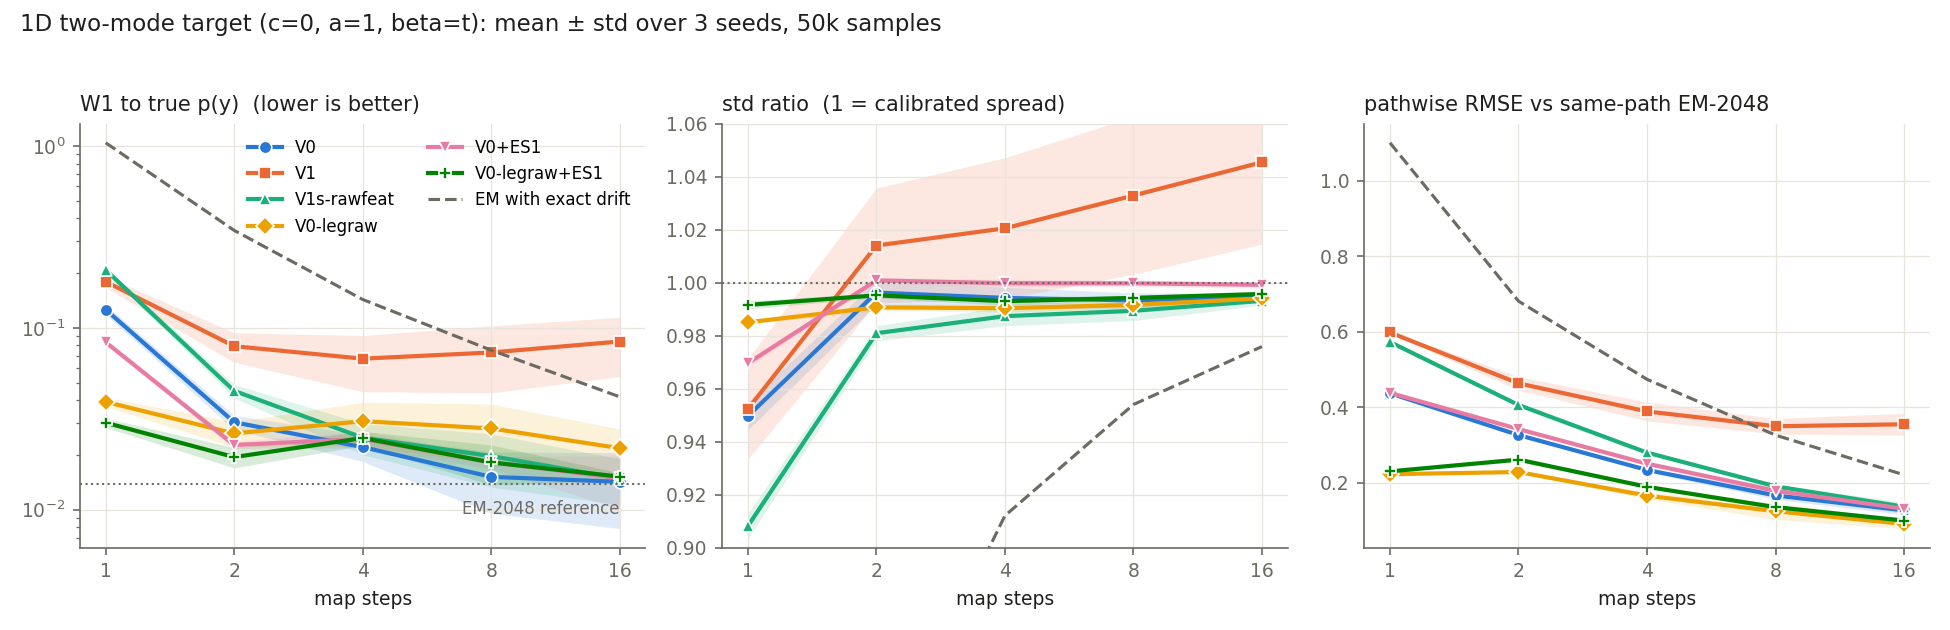
\includegraphics[width=0.95\linewidth]{fig_metrics_vs_steps.png}
\end{center}

\noindent Caveats: 1D and one 2D mixture, well-separated modes, small networks. Nothing here tests spatial spectra, the covariance-matched driver, rollouts or physics.

\section{Long rollouts}

\subsection*{D. Interpolant refresh}

\begin{center}
\includegraphics[width=\linewidth]{figures/fig_d.pdf}\\[2pt]
{\small\itshape Left: the refresh kernel. Right: fraction of a perturbation that survives one refresh, for a Gaussian mode of true spread $\sigma_f$ ($a=1$, derived values).}
\end{center}

\head{Idea.} Define the kernel $R_s$: re-noise a state $y$ to interpolant time $s$, $x_s=(1-s)c+\beta_sy+\gamma_s\sqrt s\,z$, then map back with a fresh path, $y'=\Phi_{s,1}(x_s,h;W')$. It costs one network call and is exactly what the off-diagonal loss already trains.

\head{Properties \status{derived}.}
\begin{itemize}
\item \emph{Invariance.} With exact drift, $p(\cdot\mid h)R_s=p(\cdot\mid h)$, because the interpolant and the SDE share the marginal at $s$.
\item \emph{Forgetting.} $\mathrm{KL}\big(R_s(y,\cdot)\,\|\,R_s(y+e,\cdot)\big)\le\|e\|^2s^3/(2a^2(1-s)^2)$ for $\beta=t^2$. Errors below the noise floor $a(1-s)/s^{3/2}$ are forgotten. The bound is extensive in dimension.
\item \emph{Mode-selective shrinkage.} For a Gaussian mode $\N(m,\sigma_f^2)$, $R_s$ preserves the variance and transmits a perturbation with factor $\kappa_s$. At $s=0.9$, $a=1$: $\kappa=0.38/0.64/0.93$ for $\sigma_f=0.05/0.1/0.3$. Narrow directions, where artefacts live, are pulled to the conditional mean; uncertain directions pass.
\end{itemize}

\head{Use.} \emph{Inference}: refresh every forecast before it enters the history (2 calls per physical step). \emph{Training}: replace history frames by $\sg[R_s(\text{truth frame})]$, keep the true target and the simulation-free losses. With both on, training and test histories differ only through the raw artefact, bounded by the KL above; $s$ is a continuous dial between teacher forcing and free running.

\head{Novelty.} Resampling Forcing (arXiv:2512.15702, video) does the training half without inference resampling or a guarantee. Thermalizer (arXiv:2503.18731) pulls towards the \emph{unconditional} invariant measure with a separate model. New: conditional invariance for point-base interpolants, matched use on both sides with a bound, and one-call cost.

\head{Falsifier (no training).} Roll out the 1-step map plain, as a 2-step same-path map, and with refresh at $s\in\{0.8,0.9,0.95\}$. Drop inference use if refresh does not beat the 2-step map at equal cost on spectra, enstrophy and spread against lead.

\subsection*{E. Chapman--Kolmogorov closure with direct-lead teachers}

\begin{center}
\includegraphics[width=\linewidth]{figures/fig_e.pdf}\\[2pt]
{\small\itshape Left: the composed one-step rollout is matched in law to a direct lead-$\ell$ map at the same history. Right: field autocorrelation of the data.}
\end{center}

\head{Idea.} Train the same network, with a lead embedding, as a direct lead-$\ell$ interpolant $D_\ell$ ($c\to y_{n+\ell}$). It is simulation-free and targets $p(y_{n+\ell}\mid h_n)$ exactly, with no compounding. Then make the law $A_\ell$ of $\ell$ composed one-step maps agree with it:
\[
\mathcal L=\sum_\ell w_\ell\Big[\mathrm{ES}\big(A_\ell(h),y_{n+\ell}\big)+\lambda\,\mathrm{ED}\big(A_\ell(h),\sg D_\ell(h)\big)\Big]+w_\infty\,\mathrm{ED}\big(A_L(h),\hat\mu\big),
\]
with $\ell\in\{2,3,4,6\}$ and $\hat\mu$ pooled snapshots from other trajectories, since mixing takes about 8 steps. A one-call map makes the unroll affordable; the direct kernel supplies a whole target ensemble per history instead of one truth sample, which matters with 160 training trajectories.

\head{Novelty.} The energy-score term is Swift / FGN / AIFS-CRPS and is the baseline. Neural Stochastic Flows (arXiv:2510.25769) and Kolmogorov--Chapman maps (arXiv:2611.12880) use related losses in other settings. Direct-to-autoregressive distillation in law at the same history, with the ergodic limit as the $\ell=\infty$ member, was not found.

\head{Falsifier.} One lead-conditioned run. If $D_\ell$ is not better calibrated than $A_\ell$ at $\ell=4$--$6$, drop the teacher and keep the energy score.

\subsection*{F. Stationary window matching on persistent chains}

\begin{center}
\includegraphics[width=\linewidth]{figures/fig_f.pdf}\\[2pt]
{\small\itshape Schematic. Windows of six consecutive frames from free-running model chains are matched to data windows.}
\end{center}

\head{Idea.} For an order-$p$ kernel with a unique stationary law, equality of the stationary law of $(p+1)$-frame windows implies equality of the whole stationary process; marginal invariant-measure matching does not. Here six frames also span the physical memory. Keep a buffer of free-running histories, advance it one call per iteration, and match window features (shell spectra, increment spectra, patch features) to data by energy distance, with the one-step losses kept on.

\head{Novelty.} Modest. DySLIM (arXiv:2402.04467) matches marginals of mostly deterministic emulators. Relevance is high because of the short memory.

\head{Falsifier.} Compute pooled enstrophy, spectrum, lag-1 autocorrelation (truth $0.62$) and the budget residual on the existing 4{,}096-lead runs. If all lie within the data's bootstrap band, the idea is unnecessary.

\section{Physics and other consistency}

\subsection*{G. It\^o-budget consistency}

\begin{center}
\includegraphics[width=\linewidth]{figures/fig_g.pdf}\\[2pt]
{\small\itshape Left: illustration of the budget with representative magnitudes. Right: the three budget checks on the data archive, as ratios to theory.}
\end{center}

\head{Idea.} For an SPDE the pointwise residual is the forcing and does not vanish. The right residual is the Dynkin identity for observables whose generator closes. Energy and enstrophy do, because the nonlinearity drops out.

\head{Math \status{derived, data}.} With $D=\alpha-\nu\Delta_x$ and $\mathcal W\in\{\mathrm{Id},(-\Delta_x)^{-1}\}$, a trapezoid in physical time gives
\[
\E\big[q^+_{\mathcal W}(y)\mid h\big]=q^-_{\mathcal W}(c)+\tfrac12\varepsilon^2\Delta\tr(\mathcal WQ),\qquad q^\pm_{\mathcal W}(x)=\tfrac12\langle x,\mathcal W(\mathrm{Id}\pm\Delta D)x\rangle .
\]
Since $q^+$ is quadratic,
\[
\tr\big(\mathcal W(\mathrm{Id}+\Delta D)\Cov(y\mid h)\big)=2\Big[q^-_{\mathcal W}(c)+\tfrac12\varepsilon^2\Delta\tr(\mathcal WQ)-q^+_{\mathcal W}(\E[y\mid h])\Big].
\]
Physics pins two differently weighted traces of the forecast covariance, i.e.\ the ensemble \emph{spread}. On the archive the per-pair residual has mean $-0.5\%\pm0.5\%$ of the injection, is uncorrelated with the state, and has standard deviation $0.722$ against $0.720$ predicted from the quadratic variation. Injection per step is about $1.0$ against mean enstrophy $4.78$, so the constraint is well conditioned.

\head{Uses.}
\begin{itemize}
\item \emph{Label-free diagnostic}: per member and lead, $r=q^+(y_{n+1})-q^-(y_n)-\mathrm{inj}$ must be a mean-zero martingale difference with known variance. It works beyond lead 95, where no truth exists.
\item \emph{Loss}: the unbiased U-statistic $\frac{1}{E(E-1)}\sum_{e\ne e'}r_er_{e'}$ on one-step samples. The naive $(\text{mean }r)^2$ penalises $\Var(q(y))$ and would worsen underdispersion. It needs no target, so it applies on rolled-out histories.
\item \emph{Driver scale}: $\lambda(h)$ in $C(h)=\lambda^2C_0$ of idea A.
\end{itemize}

\head{Novelty.} PIDM, DiffusionPDE, CoCoGen and PCFM use pointwise or hard residuals. The energy-consistent interpolant work (arXiv:2504.05852) budgets the interpolant in pseudo-time for a deterministic PDE. No Dynkin-type conditional-moment loss was found.

\head{Risks.} Only two scalars are constrained, and a biased mean can be compensated by wrong spread; use a small weight. It needs known $\nu,\alpha,\varepsilon,Q$.

\head{Falsifier (no training).} The known coverage deficit of It\^o maps should appear as a negative mean residual on existing rollouts.

\subsection*{H. Invariant-closed maps}

\begin{center}
\includegraphics[width=\linewidth]{figures/fig_h.pdf}\\[2pt]
{\small\itshape Left: schematic of the constrained parametrisation. Right: illustration with synthetic numbers of an invariant drifting in an unconstrained rollout.}
\end{center}

If $Ly=\ell(h)$ almost surely and $LC^{1/2}=0$, then $L\Phi_{s,t}(x)=Lx+\ell_t-\ell_s$ with $\ell_t=(1-t)Lc+\beta_t\ell(h)$. The parametrisation
\[
G_\theta=(\mathrm{Id}-L^+L)N_\theta+L^+\frac{\ell_t-\ell_s}{t-s}
\]
enforces this for every $\theta$ and every step count, and the class is closed under composition and under the self-distillation targets. With a white driver, $Lb_t$ contains the singular pull $-(Lx-\ell_t)/(1-t)$, which a few-step map cannot integrate; this is why such maps leak invariants. Here the invariant is the mean vorticity (zero to $10^{-6}$ in the data): remove $k=0$ from $C$ and from $G$. Novelty is low; the driver null-space condition and closure under self-distillation are the new parts.

\subsection*{I. Martingale Kalman conditioning}

\begin{center}
\includegraphics[width=\linewidth]{figures/fig_i.pdf}\\[2pt]
{\small\itshape Illustration on a 1D Gaussian field. The forecast ensemble is conditioned on three observations by updating each member's noise path.}
\end{center}

\head{Idea.} Maps have no trajectory to guide. But the one-step map is $y=c+G_\theta(\Psi)+S\Psi$ with a Gaussian $\Psi$ entering linearly, so observations $o=Hy+\eta$ can be imposed on the driver. Freeze $G$ and sample the linear-Gaussian posterior by Matheron's rule,
\[
\Psi^+=\Psi+(D\mathbf 1\otimes CH^\top)\big(q(1)HCH^\top+R\big)^{-1}\big(o+\tilde\eta-Hy\big),
\]
then correct exactly with preconditioned Crank--Nicolson relative to that reference, accepting on the residual likelihood. This costs one network call per step and no gradients. In the Gaussian limit of idea A the acceptance is one and samples are i.i.d.

\head{Novelty.} Pan et al.\ steer with Monte Carlo $h$-transform estimators in multi-step rollouts. D-Flow needs gradients. Source-space pCN with flow maps exists for static image priors (arXiv:2610.01034). An analytic gain from the known driver covariance, for a forecast kernel, was not found. It depends on idea A: with a white driver the frozen-Jacobian reference is poor.

\subsection*{J. Forcing-revealed latents}

\begin{center}
\includegraphics[width=\linewidth]{figures/fig_j.pdf}\\[2pt]
{\small\itshape Schematic. Logged coefficients of the physical forcing become an exactly sampled input; the generative driver models the remainder.}
\end{center}

The physical randomness is an 8-dimensional Wiener path per interval. If the regenerated dataset logs it, condition the map on a few of its chaos coefficients $\psi$ and sample them exactly at inference: $p(y\mid h)=\E_\psi p(y\mid h,\psi)$. The generative driver then models only the residual, and assimilation becomes inference over a few dozen numbers. Simulator-only falsifier: $\Var(y\mid c,\psi_{<J})/\Var(y\mid c)$ for $J=1,\dots,8$; it fails if less than $80\%$ is explained at $J\le4$. Log the forcing in the regenerated dataset regardless.

\section{Considered and discarded}\label{sec:discarded}

\begin{itemize}
\item \emph{Larger $K$ with the current local increments}: $K=16$ did not beat $K=4$ in the initial stage; change the feature type instead.
\item \emph{$(t-s)^2$ endpoint weighting}: starves short intervals and does not touch the mechanism.
\item \emph{Post-hoc variance inflation, noise temperature}: not a valid change of law; breaks spectra.
\item \emph{Eulerian / MeanFlow identities}: Pan et al.\ Prop.~2 gives zero-loss solutions that ignore $W$.
\item \emph{KL-optimal F\"ollmer process with a posterior sampler}: this is STMD / distributional diffusion; a baseline.
\item \emph{Physical-time semigroup on an extended clock}: sound, but it distils the model's own rollout; faster, not more faithful.
\item \emph{Pathwise shadowing of a finer reference across physical steps}: imposes spurious contraction given the fast decorrelation.
\item \emph{Truth as regression target on model-generated histories}: the optimum blurs for a stochastic model.
\item \emph{Brownian paths correlated across physical steps}: breaks the one-step law.
\item \emph{Noised-history conditioning}: known, and destroys small-scale information; idea D achieves the masking without it.
\item \emph{Pointwise PDE residuals}: the residual is the forcing.
\item \emph{Coupling the generative $W$ to the physical forcing inside the interpolant}: breaks the independence the drift identity needs.
\item \emph{Learning $C$ through the diagonal loss; state-dependent diffusion}: ill-posed; loses exact martingale sampling.
\item \emph{Transplanted multi-step guidance (DPS, ECI, PCFM)}: too few steps.
\item \emph{Rotation equivariance}: $90^\circ$ rotation is not a symmetry here (forcing has modes $(6,0),(7,0)$ but not $(0,6),(0,7)$); use translations and sign-flipping reflections only.
\end{itemize}

\section{Suggested order}

\begin{enumerate}
\item Run the no-training diagnostics of Section~\ref{sec:diagnosis} and the budget diagnostic (G) on existing checkpoints and rollouts. Confirm the value of $a$ used in each archived run.
\item Idea A on the SI drift only, with the nested Monte Carlo path-compression test. This is cheap and decides the direction.
\item Refresh at inference (D) on an existing one-step map.
\item Train the map on the matched process with the invariant closure (H) and nested or Legendre features; compare PSD against Picard (C).
\item Add the weak closure (B) if rank histograms stay U-shaped, with terminal CRPS as control.
\item Rollout fine-tuning: energy-score baseline against the Chapman--Kolmogorov closure (E) and refresh training (D), judged with G and F statistics.
\item Path-space assimilation (I) once A holds. Log forcing in the regenerated dataset (J).
\end{enumerate}

\appendix
\section{Provenance and caveats}\label{sec:provenance}

\begin{itemize}
\item Full agent reports, the numerical check scripts and the toy-study scripts are in \texttt{agent\_reports/} next to this file. Scripts with relative paths are run from the repository root.
\item No trained Navier--Stokes checkpoint was run. All quantitative support is from scalar or 1D toys and from statistics of the data archive.
\item The forecast-error scale ($\sigma\approx0.17$ normalised) is inferred from old CRPS values and is rough.
\item Many cited 2025--2026 papers were identified from search results or abstracts and not read in full. Verified by opening the paper: arXiv:2606.11156, 2606.01086, 2610.29605, 2611.12880, 2608.22309, 2605.07661, 2610.01034. Treat the remaining identifiers as leads to verify before citing. One discrepancy is open: iSSFM states that Pan et al.\ add the increment $W_t-W_s$ to the KL features, whereas the version of Pan et al.\ that was read says it is withheld from the network.
\item ``Not found'' means not found in the searches run, not that it does not exist.
\end{itemize}

\end{document}
